\usepackage{graphicx}
\graphicspath{ {img/} }

\chapter{Funzioni a due variabili}

\section{Generalità}

\section{Limiti}

Diciamo che $\lim_{(x,y)\to(x_0,y_0)} f(x,y) = L$ se e solo se fissato un numero reale positivo $\epsilon>0$ esiste un $\gamma>0$ tale che se $(x,y)$ appartengono all'intorno bucato di $(x_0,y_0)$ di raggio $\gamma$ allora $|f(x,y)-L|<\epsilon$

\section{Continuità}

Una funzione $f(x,y)$ si dice continua in un punto $(x_0,y_0)$ se:

\begin{itemize}
\item E' definita in $(x_0,y_0)$
\item Esiste il limite $\lim_{(x,y)\to(x_0,y_0)} f(x,y)$ ed è uguale a $f(x_0,y_0)$
\end{itemize}

Quindi non è detto che se esiste il limite di una funzione in un punto allora la funzione è definita in quel punto.

\section{Derivabilità}

\subsection{Derivata in $R$}

$$f'(x_0)=\lim_{h\to 0}\frac{f(x_0+h)-f(x_0)}{h}$$

\subsection{Derivate Parziali}

Calcolate solo rispetto all'asse $x$ o all'asse $y$.
 
\begin{figure}[h]
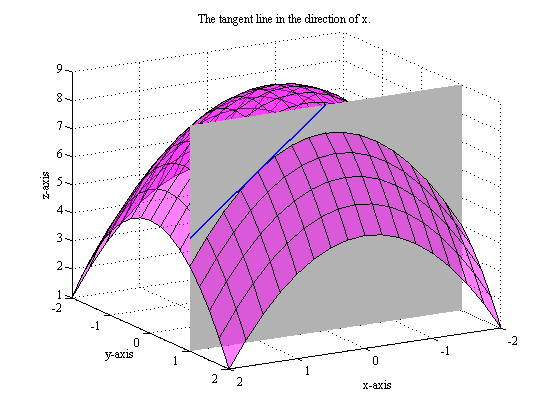
\includegraphics[width=\textwidth]{diff_partial.png}
\end{figure}

$$
f_x(x_0,y_0) = \lim_{h\to 0} \frac{f(x_0+h,y_0)-f(x_0,y_0)}{h}
$$

$$
f_y(x_0,y_0) = \lim_{k\to 0} \frac{f(x_0,y_0+k)-f(x_0,y_0)}{k}
$$

\subsection{Derivata direzionale}

Calcolata rispetto ad una qualsiasi retta/direzione.

Fissato un qualunque vettore $V=(v_1,v_2)$ non nullo posso provare a calcolare:

$$
f_v(x_0,y_0) = \lim_{h\to 0} \frac{f(x_0+v_1h,y_0+v_2h)-f(x_0,y_0)}{h}
$$

La derivata direzionale si puo' anche definire rispetto ai soli versori, cioè i vettori che hanno norma 1, visto che anche solo con questi si possono \textit{identificare} tutte le direzioni.

La derivata direzionale è anche uguale a $$\nable f(x_0,y_0)\cdot V$$

\subsection{Sviluppo di Taylor}

$$f(x,y) = f(x_0,y_0)-f_x(x_0,y_0)(x-x_0)+f_y(x_0,y_0)(y-y_0)+ \
\frac{1}{2} [f_{xx}(x_0,y_0)(x-x_0)^2+2f_{xy}(x_0,y_0)(x-x_0)(y-y_0)+f_{yy}(x_0,y_0)(y-y0)^2]+ \
o((x-x_0)^2+(y-y_0)^2)
$$

\section{Differenziabilità}

\subsection{Differenziabilità in $R$}

Una funzione $f$ è differenziabile in $x_0$ se esiste un numero $\alpha \in R$ tale che:

$$f(x_0+h)=f(x_0)+\alpha h + o(h)$$

per $h \to 0$.
 
\subsection{Generalità}

Si dice che la funzione $f(x,y)$ è differenziabile in $(x_0,y0)$ se vale che: 
$$
\lim_{(h,k)\to (0,0)} \frac{f(x_0+h,y_0+k) - f(x_0,y_0) - h A - k B}{\sqrt{h^2+k^2}} = 0
$$
dove $A=f_x(x_0,y_0)$ e $B=f_y(x_0,y_0)$

\subsection{Condizioni esistenza}

Per essere differenziabile una funzione deve essere continua e deve ammettere derivate parziali in $(a,b)$ lungo ogni direzione $V \in R^2$ (e quindi anche le derivate parziali).

\subsection{Gradiente}

Chiamiamo $\nabla f(x_0,y_0)$ il gradiente della funzione $f$ calcolato in $(x_0,y_0)$. 

$$ \nabla f(x_0,y_0) = (f_x(x_0,y_0),f_y(x_0,y_0))$$

Il vettore gradiente calcolato in un punto è anche detto \textbf{differenziale} della funzione in quel punto.

\subsubsection{Interpretazione geometrica}

\textbf{Per quali versori di $V$ la derivata direzionale risulta Massima o Minima?}

$$
f_V(x_0)  = |\nabla f(x_0)| \cdot |V| \cdot \cos(\theta)
$$

Visto che stiamo trattando versori allora $|V|=1$.

Quindi è la derivata direzionale è massima per $\cos(\theta)=1 \rightarrow \theta=0$

Quindi è la derivata direzionale è minima per $\cos(\theta)=0 \rightarrow \theta=\pi$

La direzione del gradiente calcolato in un punto indica la retta seguendo la quale si trova il massimo incremento della funzione $f$ nell'intorno del punto in cui è calcolato.

\subsection{Differenziale}

\subsubsection{Generalità}

Se le derivate prime esistono, possiamo definire il differenziale: il differenziale di una funzione quantifica la variazione infinitesimale della funzione rispetto ad una variabile indipendente.


\section{Punti di massimo e di minimo}

\subsection{Matrice Jacobiana}

La matrice jacobiana di una funzione è la matrice i cui elementi sono le derivate parziali prime della funzione.

La sua importanza è legata al fatto che, nel caso la funzione sia differenziabile, la jacobiana rappresenta la migliore approssimazione lineare della funzione vicino a un punto dato.


Sia $\mathbf{f}: U \rightarrow \mathbb R^m$ una funzione definita su un insieme aperto $U$ dello spazio euclideo  $\mathbb R^n$ . La matrice jacobiana della funzione $J {\mathbf f}$ in $\mathbf x = (x_1, \dots, x_n)$ è la matrice delle derivate parziali prime della funzione calcolate in $\mathbf x$:

$$J \, \mathbf f = \begin{bmatrix} \dfrac{\partial f_1}{\partial x_1} & \cdots & \dfrac{\partial f_1}{\partial x_n} \\ \vdots & \ddots & \vdots \\ \dfrac{\partial f_m}{\partial x_1} & \cdots & \dfrac{\partial f_m}{\partial x_n}  \end{bmatrix}\qquad \operatorname (J \, \mathbf f)_{ij} = \frac{\partial f_i (\mathbf {x})}{\partial x_j} $$

